% SOICT 2026 submission --- directed vol->PK GAT news model, v1 --- Springer LNCS format.
% Content = the finalized three-seed draft docs/paper/trackA_gat_paper_draft_3seed.md.
% All numbers, tables, and wording are transcribed verbatim from that Markdown; do not alter values.
% Template/toolchain reused from docs/paper/soict2026_trackb_v1.tex (llncs.cls, pdflatex).
% NOTE: verify llncs.cls/splncs04.bst against the official SOICT 2026 download before final submission.
% Figures are the PDF renders of docs/paper/diagrams/generate_trackA_diagrams.py
%   (trackA_gat_architecture.pdf, trackA_gat_ablation.pdf).
%
\documentclass[runningheads]{llncs}
%
\usepackage[T1]{fontenc}
\usepackage{graphicx}
\usepackage{amsmath}
\usepackage{amssymb}
\usepackage{booktabs}
%
\begin{document}
%
\title{Stock Volatility Prediction for the Vietnamese Stock Market}
%
\titlerunning{Volatility Prediction for the Vietnamese Stock Market}
%
% TODO(authors): fill in the real author names, affiliations, and e-mail addresses before submission.
\author{Author One\inst{1} \and Author Two\inst{1}}
\authorrunning{Author One et al.}
%
\institute{VNUHCM University of Science, Ho Chi Minh City, Vietnam\\
\email{\{author1,author2\}@student.hcmus.edu.vn}}
%
\maketitle
%
\begin{abstract}
Volatility forecasts set risk limits, margin, and option prices across the Vietnamese stock market. This
work targets volatility forecasting for Vietnamese equities in general and uses the VN30 constituents
(the most liquid stocks on Vietnam's Ho Chi Minh Stock Exchange) as the empirical case study. Two
structural signals a univariate Heterogeneous AutoRegressive (HAR) model discards are Vietnamese-language
news and cross-stock spillover. We propose a parallel multi-branch model that fuses three branches for one
ticker's multi-horizon Parkinson-variance forecast: a per-node price LSTM over five node features, a real
multi-head Graph Attention Network (GAT) over a directed volume-to-volatility (vol$\to$PK) lead-lag edge,
and a PhoBERT news LSTM with a per-ticker gate. The GAT branch consumes the raw node-feature vector at the
forecast origin rather than the LSTM hidden state, which matches the edge semantics (a source ticker's
volume shock at $t$ leading a target ticker's volatility at $t{+}1$) and keeps the graph branch an
independent cross-sectional view for a fair ablation. We evaluate the model with an ablation: from the full
model we retrain one variant per removed component (minus-graph removes the entire GAT branch, minus-gate
removes the per-ticker gate, minus-news removes the news branch), and we measure each component's
contribution as $\text{effect}(X)=\text{QLIKE}(\text{FULL})-\text{QLIKE}(\text{FULL}{-}X)$ on the held-out
test set, with a Diebold--Mariano test for significance. The classical HAR is the reference baseline.
Across three seeds and four horizons the differences among HAR, the full model, and the ablation variants
are small on every metric. On MSE, RMSE, and $R^2$ the configuration means lie within about 1\% of one
another and the best mean alternates across horizons; on MAE the differences are similarly small and the
lowest mean varies by horizon. On QLIKE, HAR has the lowest mean at h5, h10, and h22 and the price-only
LSTM backbone the lowest at h1. Diebold--Mariano tests on the seed-ensembled predictions, run on the
QLIKE, squared-error, and absolute-error loss families, show no model favored across all three: relative
to HAR the full model shows no significant QLIKE difference at h1, h5, and h10 and significantly higher
QLIKE at h22, no significant squared-error difference at any horizon, and significantly lower absolute-error
loss at h5. The ablation removals are significant on some loss families and horizons and not others, so no
ablation verdict holds uniformly across the three losses and four horizons. Across all five metrics no
configuration consistently or significantly outperforms HAR. This paper's contribution is a leakage-safe
ablation-based attribution of a directed-spillover graph-attention news model against a strong HAR baseline
on sparse daily VN30 data.

\keywords{Volatility forecasting \and Graph attention networks \and Directed spillover \and Financial news
\and PhoBERT \and Emerging markets.}
\end{abstract}
%
% ======================================================================
\section{Introduction}
\label{sec:intro}
Volatility forecasts drive the daily risk decisions of every desk that trades Vietnamese equities. This
work addresses stock-volatility forecasting for the Vietnamese market in general; the VN30 basket (the
roughly thirty most liquid stocks on Vietnam's Ho Chi Minh Stock Exchange) is the empirical case study
used for all experiments because it has the longest and cleanest daily histories. A margin engine sizes
collateral from forecast volatility, an option desk prices from it, and a risk officer sets position limits
against it. VN30 desks make these decisions inside an information environment that a price-only forecaster
discards: a steady flow of Vietnamese-language news that plausibly signals volatility shocks before they
reach the price range, and a web of cross-stock spillovers that a univariate model cannot represent.

The classical HAR model of Corsi~\cite{corsi2009}, the linear univariate workhorse that regresses future
volatility on its own daily, weekly, and monthly averages, admits neither signal, and it is hard to
beat~\cite{audrino2025}. Two structural extensions could close the gap: a news channel that reads text, and
a cross-stock graph that lets one stock's information reach another. Prior work on this project
established, through a leakage-safe exploratory analysis, that adding cross-sectional node features (a
market factor and a volume z-score) beats HAR on QLIKE, but that a \emph{correlation-based} cross-stock
edge adds no reliable out-of-sample value because a single market factor dominates cross-stock volatility
co-movement. This motivates the present study's central design choice: rather than a symmetric correlation
edge, we test a directed, lead-lag volume$\to$volatility edge --- a source ticker's abnormal volume today
linked to a target ticker's range volatility tomorrow --- which encodes a predictive, causal-direction
relationship that a contemporaneous correlation edge cannot.

We build this edge into a parallel multi-branch architecture (an LSTM temporal branch, a GAT graph branch,
and a gated news branch, concatenated at a shared head) and we quantify, per component and per horizon, the
marginal contribution of each part with an ablation: we build the full model, then retrain a variant with
exactly one component removed, and attribute each component's contribution as the change in held-out QLIKE
it causes. This paper makes three contributions.
\begin{enumerate}
\item \textbf{A directed vol$\to$PK graph-attention news model on a parallel multi-branch backbone.} The
model fuses a per-node price LSTM, a real multi-head GAT over a directed volume-to-volatility lead-lag edge,
and a gated PhoBERT news branch. The GAT consumes the raw node-feature vector at the forecast origin, which
matches the edge semantics and keeps the graph branch an independent cross-sectional view
(Section~\ref{sec:method}).
\item \textbf{An ablation against a strong HAR baseline.} From the full model we retrain one variant per
removed component --- minus-graph (the whole GAT branch), minus-gate, minus-news --- so every effect is
measured on the same footing, and we report each component's marginal contribution
$\text{effect}(X)=\text{QLIKE}(\text{FULL})-\text{QLIKE}(\text{FULL}{-}X)$ with a Diebold--Mariano test
(Section~\ref{sec:results}).
\item \textbf{A leakage-safe multi-horizon evaluation.} All models are evaluated at horizons 1, 5, 10, and
22 trading days on a chronological split with train-only scalers and a train-only frozen edge, with the
held-out test set as the reported result, over three seeds with seed-ensembled significance tests
(Sections~\ref{sec:setup} and~\ref{sec:results}).
\end{enumerate}

% ======================================================================
\section{Related Work}
\label{sec:related}
We group prior work into four families and state where the proposed model sits relative to each.

\subsubsection{Econometric volatility models.}
The HAR model~\cite{corsi2009} and its range-based inputs~\cite{parkinson1980} set the standard for daily
volatility forecasting and remain hard to beat. HAR regresses future volatility on daily, weekly, and
monthly moving averages, approximating volatility's long memory with a parsimonious linear fit. The HARQ
extension~\cite{bpq2016} shrinks the daily coefficient when the volatility estimate is noisy. A large-scale
controlled study finds that tuned machine-learning models fail to beat a carefully re-estimated HAR on
QLIKE and MSE when both use the same information set~\cite{audrino2025}. These models are univariate and
linear: no channel admits text, and no channel couples one stock to another. We keep the three HAR scales
among the node features and add the news and directed cross-stock channels HAR omits; classical HAR is the
baseline every component must beat.

\subsubsection{Deep and graph-based forecasters.}
LSTM forecasters~\cite{hochreiter1997} capture nonlinear temporal structure, and graph attention
networks~\cite{velickovic2018} model cross-asset coupling; hybrid LSTM-GNN designs combine
both~\cite{sonani2025}. Chen and Robert~\cite{chen2022} forecast multivariate realized volatility with a
graph over about 500 S\&P names. Most relevant, Zhang, Pu, Cucuringu and Dong~\cite{zhang2025gnnhar} build a
graph-neural-network HAR (GNNHAR) on DJIA-30 and, under a Model Confidence Set, find that multi-hop
cross-stock graph spillover gives no clear advantage: the gains come from modeling nonlinearity and from
switching the training loss from MSE to QLIKE. Their controlled null on the graph component motivates our
shift from a symmetric correlation edge to a directed lead-lag edge, tested here under an ablation.

\subsubsection{Directed spillover and lead-lag graphs.}
A symmetric correlation edge conflates contemporaneous co-movement (largely a market factor) with
predictive structure. Directed spillover measures --- for example volatility spillover
indices~\cite{diebold2012} --- encode who-leads-whom and are asymmetric by construction. We instantiate a
directed edge from a source ticker's abnormal volume to a target ticker's next-day range volatility,
motivated by the volume--volatility lead-lag relation, and freeze it on the training window.

\subsubsection{News- and text-augmented forecasting.}
Text-augmented forecasters add sentiment scores or news embeddings~\cite{ouyang2021,das2024}, usually
fusing a single market-wide signal by concatenation on English- or Chinese-language markets. We work in
Vietnamese with PhoBERT~\cite{phobert2020} on VN30 and add a per-ticker gate that admits a different amount
of news per stock.

% ======================================================================
\section{Data}
\label{sec:data}
\subsubsection{Universe (case study).}
The method targets the Vietnamese stock market in general; VN30 is the case-study universe for the
experiments. We use 33 VN30 constituents with daily open-high-low-close-volume (OHLCV) data. Series lengths
range from about 1{,}300 sessions (SSB, listed 2021) to about 4{,}900 (VNM, ACB, from 2006). The universe
is a fixed, point-in-time VN30-like set rather than the live index, a limitation stated in the Limitations
section.

\subsubsection{Forecast target.}
We forecast the daily Parkinson range volatility at horizons 1, 5, 10, and 22 trading days ahead: the
target is the single-day estimator value on day $t{+}h$ (i.e.\ $\text{PK}(t{+}h)$), not an average over
the next $h$ days. The Parkinson estimator uses the intraday high $H$ and low $L$:
\begin{equation}
\sigma^2_{\text{Park}} = \frac{(\ln(H/L))^2}{4\ln 2}.
\label{eq:parkinson}
\end{equation}
The processed \texttt{parkinson\_volatility} column is numerically the Parkinson \textbf{variance}
estimator ($\sigma^2$, non-negative), and every model in this paper forecasts this same daily
realized-variance quantity.

\subsubsection{Node features.}
Each ticker-day carries five node features in a fixed order, all with unified 22-trading-day windows to
match the monthly HAR scale:
\begin{enumerate}
\item \texttt{pk\_daily} --- the Parkinson variance at $t$, clipped to $\pm 3\sigma$ using train statistics.
\item \texttt{har\_weekly} --- trailing 5-day mean of \texttt{pk\_daily}.
\item \texttt{har\_monthly} --- trailing 22-day mean of \texttt{pk\_daily}.
\item \texttt{market\_pk} --- cross-sectional median of $\sqrt{\text{PK}}$ across present tickers at $t$ (a
contemporaneous market factor; uses column $t$ only).
\item \texttt{volume\_zscore} --- trailing rolling-22 z-score of $\log(1+\text{volume})$; tickers with no
OHLCV volume series receive a neutral $0.0$.
\end{enumerate}

\subsubsection{News panel.}
Each Vietnamese article (title and lead) passes once through PhoBERT~\cite{phobert2020}, yielding a
768-dimensional embedding reduced by PCA (fit before the training cutoff) to a per-day per-stock vector of
146 dimensions (embedding components, per-group norms, exponentially weighted averages with a
30-trading-day half-life, and topic counts). Missing news on a day is a zero vector with a mask bit set to
zero, and an all-missing window still produces a finite representation.

\subsubsection{Directed vol$\to$PK edge.}
The adjacency is directed: for each target ticker $j$ we connect the Top-5 source tickers $i$ ranked by the
train-only lead-lag correlation
$\text{corr}(\text{volume\_shock}_i(t),\ \sqrt{\text{PK}_j}(t{+}1))$. Edges are estimated on training rows
only and frozen for validation and test (leakage-safe), and self-loops are kept on the diagonal.

\subsubsection{Temporal split and leakage control.}
Each ticker's series is split chronologically into 70\% train, 15\% validation, and 15\% test before
generating features, fitting scalers, or building windows; the earliest series begin in 2006. The split is
applied per ticker on its own timeline, so the train/validation/test calendar boundaries differ across
tickers --- a ticker listed in 2021 has later boundaries than one trading since 2006 --- which is precisely
why a fixed-node synchronized panel would collapse and why the pooled per-ticker split is used. Per-ticker
price and target scalers are fit on the training partition only and selected at evaluation by explicit
\texttt{ticker\_id}. A news feature for a sample uses only information available by that sample's forecast
origin. Evaluation reads stored raw targets rather than inverse-transforming a clipped normalized target.
On the pooled masked manifest the evaluation sets hold, at the five-day horizon, 14{,}418 validation and
14{,}464 present-node test observations, shared identically across every rung; the counts vary slightly by
horizon (e.g.\ 14{,}550/14{,}596 at h1 and 14{,}253/14{,}299 at h10) because the target shift changes the
number of eligible windows.

% ======================================================================
\section{Method}
\label{sec:method}
We describe the proposed full model first, then define the ablation variants as component removals from it.
The model forecasts one ticker's $h$-day-ahead Parkinson variance from four inputs: a 22-day price window
of the five node features, a 22-day news window of PhoBERT features with a mask, the ticker identity, and
the directed vol$\to$PK adjacency over the tickers present on the same date.

\begin{figure}[t]
\centering
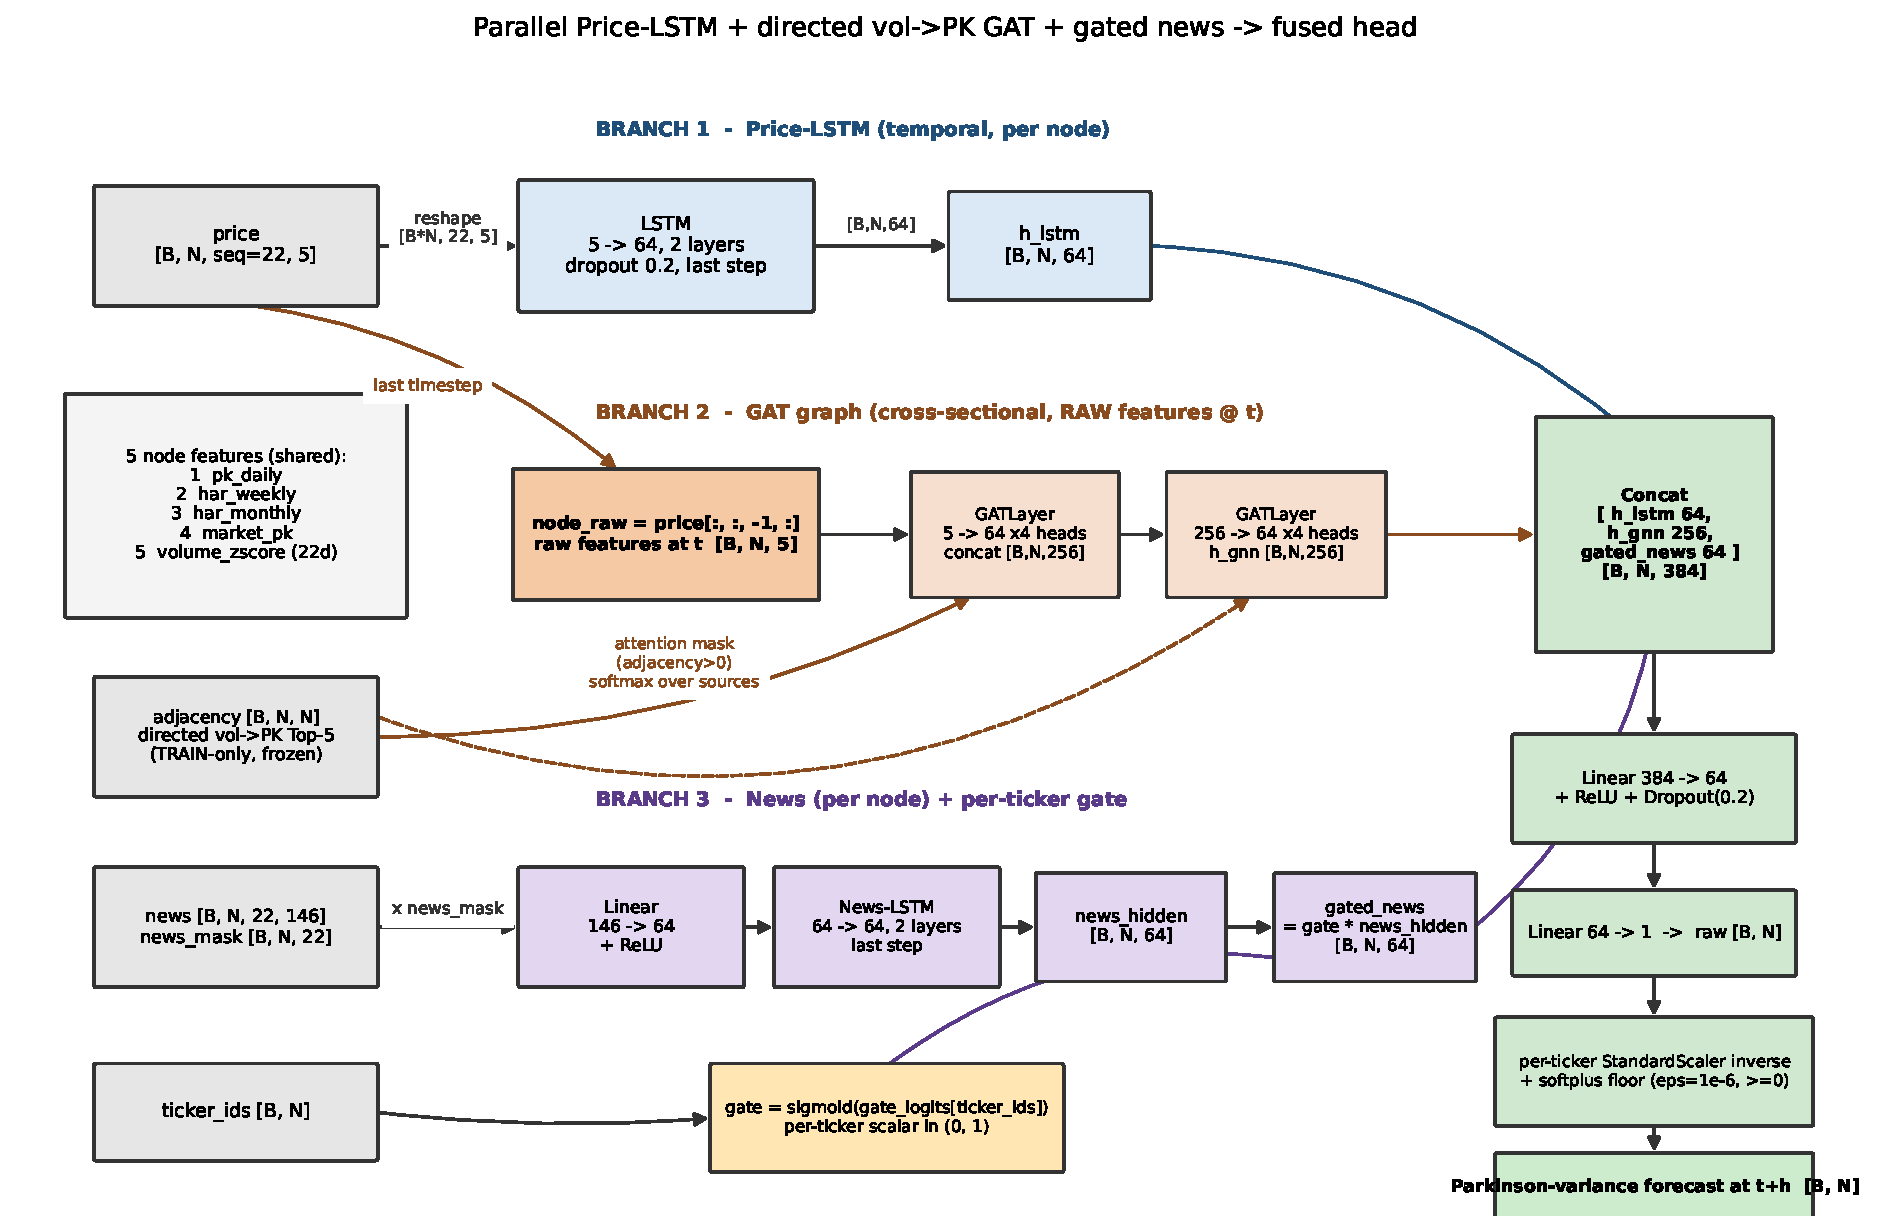
\includegraphics[width=\textwidth]{diagrams/trackA_gat_architecture.pdf}
\caption{Model architecture: parallel price-LSTM, directed vol$\to$PK GAT (on raw node features), and gated
PhoBERT news branches, concatenated into a head with a softplus positivity floor.}
\label{fig:arch}
\end{figure}

\noindent\textbf{The proposed full model.} Three branches run in parallel and concatenate at a shared head.
\begin{itemize}
\item \textbf{(i) Price-LSTM branch (temporal, per node).} A two-layer LSTM (hidden size 64, dropout 0.2)
reads each ticker's 22-day window of the five node features into a price representation $h_{\text{lstm}}$
($\mathbb{R}^{64}$ per node).
\item \textbf{(ii) GAT graph branch (cross-sectional).} The node input is the \textbf{raw} node-feature
vector at the last timestep, $\text{node\_raw}=\text{price}[:, :, {-}1, :]\in\mathbb{R}^{5}$, not the LSTM
hidden state. Two self-written multi-head GAT layers ($5\to256$, then $256\to256$; 4 heads) with attention
masked by the adjacency ($\text{softmax}$ over source nodes, ELU output) produce
$h_{\text{gnn}}\in\mathbb{R}^{256}$. Consuming the raw features matches the edge semantics
(\texttt{volume\_shock} is directly available to the attention) and keeps the graph branch independent of
the LSTM branch, so removing it is a clean ablation. When the graph is switched off, the adjacency is the
identity (self-loops only).
\item \textbf{(iii) News branch with per-ticker gate.} The 146-dimensional daily news vector passes through
a linear-plus-ReLU projection into a two-layer LSTM (hidden size 64) over the masked window, producing a
news representation, scaled by a learned per-ticker sigmoid gate
$\text{news}^{\text{gated}}_i = \sigma(g_i)\cdot\text{news}_i$.
\end{itemize}
The head concatenates $[h_{\text{lstm}}(64),\ h_{\text{gnn}}(256),\ \text{news}^{\text{gated}}(64)]$
($\mathbb{R}^{384}$) and maps it through a linear-ReLU-dropout-linear stack to the forecast. A softplus
\textbf{positivity floor} ($\varepsilon=10^{-6}$, applied in the denormalized space and identical across
all compared rungs) clamps predictions away from non-positive variance before QLIKE.

\begin{figure}[t]
\centering
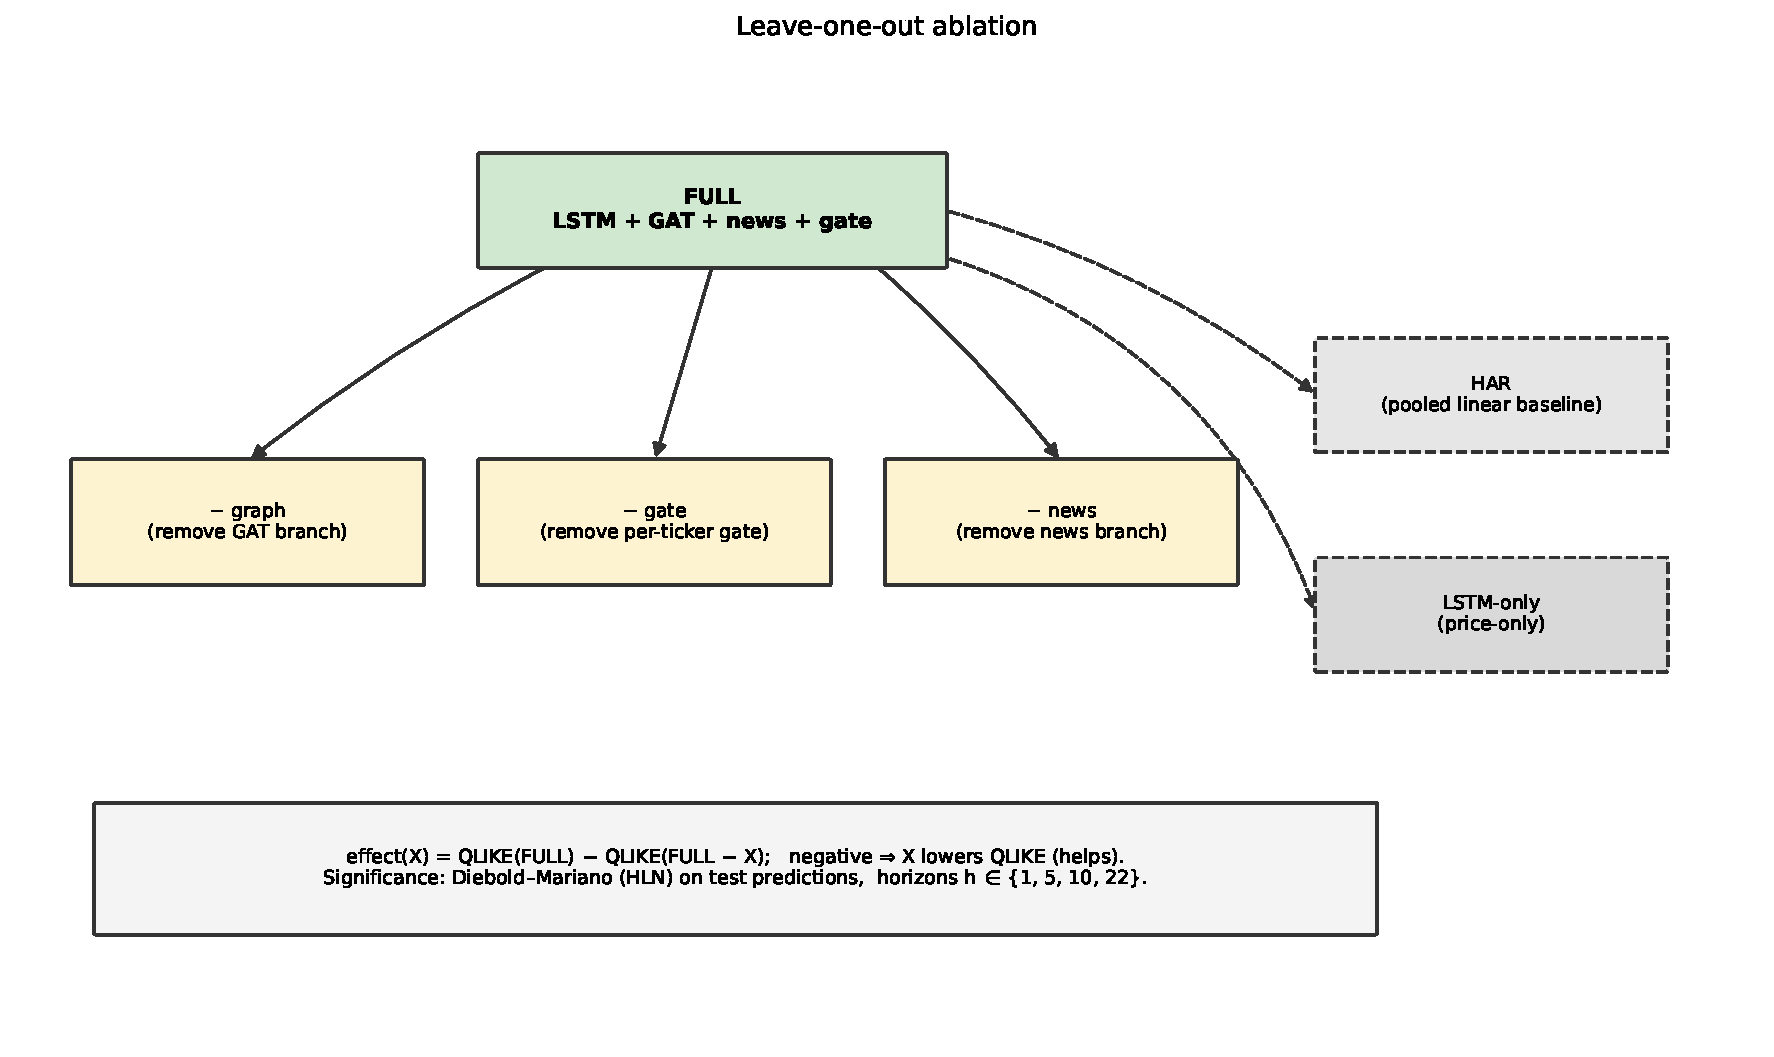
\includegraphics[width=\textwidth]{diagrams/trackA_gat_ablation.pdf}
\caption{Ablation: from FULL, one component is removed per variant ($-$graph, $-$gate, $-$news); HAR and a
price-only LSTM-only model are reference baselines.
$\text{effect}(X)=\text{QLIKE}(\text{FULL})-\text{QLIKE}(\text{FULL}{-}X)$.}
\label{fig:ablation}
\end{figure}

\noindent\textbf{The ablation variants.} We build the full model, then retrain one variant per removed
component, so every effect is measured on the same footing (each variant trains in the same graph on/off
regime it is evaluated in --- no train/eval mismatch):
\begin{itemize}
\item \textbf{FULL} --- LSTM + directed vol$\to$PK GAT graph + news + per-ticker gate.
\item \textbf{$-$graph} --- FULL with the \textbf{entire GAT branch removed} (no node/edge/GAT built; the
head takes $[h_{\text{lstm}},\ \text{news}^{\text{gated}}]\in\mathbb{R}^{128}$). This isolates the whole
graph subsystem, not merely the edges.
\item \textbf{$-$gate} --- FULL without the per-ticker gate.
\item \textbf{$-$news} --- FULL without the news branch (the gate is a no-op without news).
\item \textbf{HAR} --- a pooled per-ticker HAR linear regression on the three HAR scales; the floor every
component must beat.
\end{itemize}
The contribution of component $X$ is
$\text{effect}(X)=\text{QLIKE}(\text{FULL})-\text{QLIKE}(\text{FULL}{-}X)$ on the held-out test set; a
negative value means removing $X$ raised QLIKE, i.e.\ $X$ helped.

\noindent\textbf{Training.} The deep models use Adam (learning rate $10^{-3}$), weight decay $10^{-5}$,
dropout 0.2, and gradient clipping at 1.0, with best-validation-checkpoint selection. Because pooled models
converge within a few epochs and then overfit, training uses early stopping (patience 3, minimum 6 epochs)
under a 12-epoch cap. Every configuration is trained under three seeds (42, 123, 2026); test metrics are
reported as mean(std) over the three seeds, and Diebold--Mariano tests run on the seed-ensembled test
predictions.

% ======================================================================
\section{Experimental Setup}
\label{sec:setup}
\subsubsection{Metrics.}
Every configuration reports five metrics on the raw variance scale: MSE, RMSE, MAE, $R^2$, and QLIKE.
QLIKE, the quasi-likelihood loss standard in the realized-volatility literature~\cite{patton2011},
penalizes under-prediction more than over-prediction and tolerates the noise in the volatility proxy:
\begin{equation}
\text{QLIKE} = \frac{1}{T}\sum_{t=1}^{T}\left(\frac{\hat{\sigma}^2_t}{\sigma^2_t}
 - \ln\frac{\hat{\sigma}^2_t}{\sigma^2_t} - 1\right).
\label{eq:qlike}
\end{equation}
Directional accuracy is not reported; the Limitations section notes why it is uninformative for this
target.

\subsubsection{Training objective.}
All deep configurations minimize the mean squared error between the model output and the per-ticker
normalized target; QLIKE and the other metrics are computed only at evaluation, after inverting the
normalization to the raw variance scale, so the proportional QLIKE loss never enters the gradient.

\subsubsection{Reporting protocol.}
Model selection (early-stopping, best-checkpoint) uses the validation split only; all reported results and
significance tests are computed on the held-out test set; validation is used only for model selection, and
no validation metrics are reported.

\subsubsection{Significance.}
We complement metric comparisons with a Diebold--Mariano (DM) test on the per-observation QLIKE (and
squared-error) loss series (HAC truncation lag $h{-}1$, Harvey--Leybourne--Newbold corrected), which tests
forecast-accuracy equality directly on the held-out observations. The DM test runs on the seed-ensembled
predictions (the per-observation mean forecast over seeds 42, 123, 2026).

\subsubsection{Implementation and compute.}
All models are implemented in PyTorch (self-written GAT layer; no external graph library) and use a CUDA
GPU. Runs used an NVIDIA GeForce RTX~4060 Laptop GPU under PyTorch~2.6 with CUDA~12.4.

% ======================================================================
\section{Results}
\label{sec:results}

\subsection{Held-out test metrics across horizons}
\label{sec:results-metrics}
Table~\ref{tab:metrics} reports the held-out test metrics by horizon, mean(std) over three seeds
(42, 123, 2026). Lower is better for MSE, RMSE, MAE, QLIKE; higher for $R^2$. Bold marks the best mean per
column within each horizon; the same test observations are shared across all rows of a horizon. HAR is a
deterministic linear regression (std $0.00$).

\begin{table}[t]
\caption{Held-out TEST metrics by horizon, mean(std) over three seeds (42, 123, 2026). Lower is better for
MSE, RMSE, MAE, QLIKE; higher for $R^2$. Bold marks the best mean per column within each horizon.}
\label{tab:metrics}
\centering
\begin{tabular}{lccccc}
\toprule
Config & MSE ($\times10^{-6}$) $\downarrow$ & RMSE ($\times10^{-3}$) $\downarrow$
 & MAE ($\times10^{-4}$) $\downarrow$ & $R^2$ $\uparrow$ & QLIKE $\downarrow$ \\
\midrule
\multicolumn{6}{l}{\emph{h $=$ 1 trading day}} \\
HAR         & 4.05 (0.00) & 2.014 (0.000) & 5.41 (0.00) & 0.8192 (0.0000) & 0.4813 (0.0000) \\
FULL        & 4.06 (0.08) & 2.015 (0.020) & 5.45 (0.07) & 0.8189 (0.0036) & 0.4853 (0.0059) \\
$-$graph    & 4.04 (0.05) & 2.009 (0.012) & 5.41 (0.05) & 0.8200 (0.0022) & 0.4797 (0.0045) \\
$-$gate     & 4.02 (0.10) & 2.006 (0.025) & 5.42 (0.06) & 0.8206 (0.0045) & 0.4830 (0.0070) \\
$-$news     & \textbf{4.01 (0.08)} & \textbf{2.003 (0.021)} & 5.42 (0.06) & \textbf{0.8210 (0.0037)} & 0.4824 (0.0071) \\
LSTM-only   & 4.08 (0.09) & 2.021 (0.022) & \textbf{5.36 (0.05)} & 0.8179 (0.0040) & \textbf{0.4791 (0.0051)} \\
\midrule
\multicolumn{6}{l}{\emph{h $=$ 5 trading days}} \\
HAR         & 5.23 (0.00) & 2.287 (0.000) & 6.05 (0.00) & 0.7672 (0.0000) & \textbf{0.5735 (0.0000)} \\
FULL        & 5.19 (0.08) & 2.278 (0.018) & \textbf{5.97 (0.05)} & 0.7691 (0.0036) & 0.5768 (0.0033) \\
$-$graph    & 5.19 (0.05) & 2.278 (0.011) & \textbf{5.97 (0.06)} & 0.7691 (0.0022) & 0.5781 (0.0064) \\
$-$gate     & \textbf{5.18 (0.05)} & 2.277 (0.012) & \textbf{5.97 (0.04)} & 0.7693 (0.0024) & 0.5757 (0.0015) \\
$-$news     & 5.21 (0.09) & 2.282 (0.019) & \textbf{5.97 (0.06)} & 0.7682 (0.0038) & 0.5759 (0.0031) \\
LSTM-only   & \textbf{5.18 (0.05)} & \textbf{2.275 (0.012)} & 5.98 (0.07) & \textbf{0.7696 (0.0024)} & 0.5772 (0.0056) \\
\midrule
\multicolumn{6}{l}{\emph{h $=$ 10 trading days}} \\
HAR         & 5.56 (0.00) & 2.358 (0.000) & 6.30 (0.00) & 0.7532 (0.0000) & \textbf{0.6139 (0.0000)} \\
FULL        & 5.56 (0.12) & 2.357 (0.026) & \textbf{6.29 (0.10)} & 0.7534 (0.0054) & 0.6441 (0.0342) \\
$-$graph    & 5.50 (0.08) & 2.345 (0.017) & 6.35 (0.03) & 0.7560 (0.0035) & 0.6179 (0.0033) \\
$-$gate     & \textbf{5.49 (0.03)} & 2.344 (0.006) & 6.34 (0.10) & 0.7562 (0.0012) & 0.6225 (0.0033) \\
$-$news     & 5.55 (0.12) & 2.356 (0.025) & 6.31 (0.14) & 0.7535 (0.0053) & 0.6595 (0.0533) \\
LSTM-only   & \textbf{5.49 (0.05)} & \textbf{2.342 (0.011)} & 6.33 (0.04) & \textbf{0.7566 (0.0023)} & 0.6189 (0.0043) \\
\midrule
\multicolumn{6}{l}{\emph{h $=$ 22 trading days}} \\
HAR         & \textbf{6.02 (0.00)} & \textbf{2.453 (0.000)} & 6.56 (0.00) & \textbf{0.7303 (0.0000)} & \textbf{0.6742 (0.0000)} \\
FULL        & 6.11 (0.03) & 2.472 (0.006) & 6.54 (0.07) & 0.7262 (0.0014) & 0.7053 (0.0066) \\
$-$graph    & 6.15 (0.14) & 2.479 (0.028) & \textbf{6.53 (0.02)} & 0.7245 (0.0062) & 0.6956 (0.0140) \\
$-$gate     & 6.22 (0.18) & 2.493 (0.037) & 6.62 (0.05) & 0.7214 (0.0082) & 0.7058 (0.0079) \\
$-$news     & 6.19 (0.09) & 2.489 (0.018) & 6.60 (0.01) & 0.7225 (0.0041) & 0.7097 (0.0107) \\
LSTM-only   & 6.09 (0.02) & 2.468 (0.004) & 6.54 (0.05) & 0.7271 (0.0009) & 0.7003 (0.0067) \\
\bottomrule
\end{tabular}
\end{table}

Reading across horizons: on the squared-error metrics (MSE, RMSE, $R^2$) the configuration means fall
within about 1\% of one another and the best row alternates ($-$news at h1, $-$gate/LSTM-only at h5/h10,
HAR at h22); on MAE the differences are similarly small and the lowest mean varies by horizon (LSTM-only at
h1, four configurations tied near 5.97 at h5, FULL at h10, $-$graph at h22); on QLIKE, HAR has the lowest
mean at h5, h10, and h22 while the price-only LSTM-only has the lowest mean at h1. The reported standard
deviations are small relative to the between-configuration gaps except at h10, where the FULL and $-$news
QLIKE means carry larger seed dispersion (std 0.034 and 0.053). The remaining subsections isolate each
component (Section~\ref{sec:results-effects}), compare FULL against HAR (Section~\ref{sec:results-fullhar}),
and test significance (Section~\ref{sec:results-dm}).

\subsection{Component contributions across horizons}
\label{sec:results-effects}
Table~\ref{tab:effects} reports each component's contribution on held-out test QLIKE,
$\text{effect}(X)=\text{QLIKE}(\text{FULL})-\text{QLIKE}(\text{FULL}{-}X)$, three-seed mean. Negative $=$
removing $X$ raised QLIKE, i.e.\ $X$ helped.

\begin{table}[t]
\caption{Component contribution on held-out test QLIKE,
$\text{effect}(X)=\text{QLIKE}(\text{FULL})-\text{QLIKE}(\text{FULL}{-}X)$, three-seed mean. Negative $=$
removing $X$ raised QLIKE, i.e.\ $X$ helped.}
\label{tab:effects}
\centering
\begin{tabular}{cccc}
\toprule
Horizon & effect(graph) & effect(gate) & effect(news) \\
\midrule
1  & $+0.00566$ & $+0.00235$ & $+0.00297$ \\
5  & $-0.00130$ & $+0.00105$ & $+0.00088$ \\
10 & $+0.02617$ & $+0.02159$ & $-0.01541$ \\
22 & $+0.00979$ & $-0.00041$ & $-0.00432$ \\
\bottomrule
\end{tabular}
\end{table}

Reading: \texttt{effect(graph)} is positive at h1, h10, and h22 (removing the GAT branch lowers QLIKE
there) and marginally negative at h5 ($-0.0013$). \texttt{effect(gate)} is positive at h1, h5, and h10 and
marginally negative at h22 ($-0.0004$). \texttt{effect(news)} is positive at h1 and h5 and negative at h10
($-0.0154$) and h22 ($-0.0043$), so removing the news branch raises QLIKE only at the longer horizons.
These are QLIKE effects; the corresponding MSE, RMSE, and $R^2$ differences among the same configurations
are within about 1\% (Table~\ref{tab:metrics}). The magnitudes at h10 are the largest, but the seed
dispersion at h10 (Table~\ref{tab:metrics}) is also the largest; the Diebold--Mariano test
(Section~\ref{sec:results-dm}) determines which differences are significant on the seed-ensembled
predictions.

\subsection{FULL versus HAR across horizons}
\label{sec:results-fullhar}
Table~\ref{tab:fullhar} pairs each metric HAR-then-FULL on the held-out test set for all four horizons,
mean(std) over three seeds; bold marks the better mean of the pair.

\begin{table}[t]
\caption{FULL vs HAR, held-out test, all four horizons, mean(std) over three seeds. Columns pair each
metric HAR-then-FULL; bold marks the better mean of the pair.}
\label{tab:fullhar}
\centering
\begin{tabular}{ccccccc}
\toprule
Horizon & HAR QLIKE & FULL QLIKE & HAR $R^2$ & FULL $R^2$
 & HAR RMSE ($\times10^{-3}$) & FULL RMSE ($\times10^{-3}$) \\
\midrule
1  & \textbf{0.4813 (0.0000)} & 0.4853 (0.0059) & \textbf{0.8192 (0.0000)} & 0.8189 (0.0036) & \textbf{2.014 (0.000)} & 2.015 (0.020) \\
5  & \textbf{0.5735 (0.0000)} & 0.5768 (0.0033) & 0.7672 (0.0000) & \textbf{0.7691 (0.0036)} & 2.287 (0.000) & \textbf{2.278 (0.018)} \\
10 & \textbf{0.6139 (0.0000)} & 0.6441 (0.0342) & 0.7532 (0.0000) & \textbf{0.7534 (0.0054)} & 2.358 (0.000) & \textbf{2.357 (0.026)} \\
22 & \textbf{0.6742 (0.0000)} & 0.7053 (0.0066) & \textbf{0.7303 (0.0000)} & 0.7262 (0.0014) & \textbf{2.453 (0.000)} & 2.472 (0.006) \\
\bottomrule
\end{tabular}
\end{table}

Reading: on RMSE and $R^2$ the full model and HAR are within their seed dispersion at h1, h5, and h10, and
HAR is marginally ahead at h22 (MSE and MAE follow the same pattern in Table~\ref{tab:metrics}). On QLIKE,
HAR has the lower mean at all four horizons, with the gap widening from h1 (0.0040) to h22 (0.0311). The
Diebold--Mariano table (Table~\ref{tab:dm}) tests these gaps across loss families on the seed-ensembled
predictions: on QLIKE the full model shows no significant difference from HAR at h1, h5, and h10 and HAR is
significantly lower at h22; on squared error there is no significant difference at any horizon; on absolute
error the full model is significantly lower at h5.

\subsection{Diebold--Mariano significance across metrics}
\label{sec:results-dm}
Table~\ref{tab:dm} reports the Diebold--Mariano (HLN) test on the held-out test set, seed-ensembled
(42, 123, 2026), per horizon and per loss family. Each cell is the HLN-corrected DM statistic with its
two-sided $p$-value; bold marks $p<0.05$. A \emph{negative} statistic means FULL has the lower loss; a
\emph{positive} statistic means the comparator has the lower loss. DM is run on three per-observation loss
families: QLIKE, squared error (SE; the MSE/RMSE/$R^2$ family), and absolute error (AE; MAE). HAC
truncation lag $h{-}1$; $n$ per horizon is 14{,}596 (h1), 14{,}464 (h5), 14{,}299 (h10), 13{,}903 (h22).

\begin{table}[t]
\caption{Diebold--Mariano (HLN) on held-out test, seed-ensembled (42, 123, 2026), per horizon and per loss
family. Cell $=$ HLN-corrected DM statistic ($p$-value); bold marks $p<0.05$. Negative statistic $=$ FULL
lower loss; positive $=$ comparator lower loss. HAC truncation lag $h{-}1$.}
\label{tab:dm}
\centering
\begin{tabular}{lccc}
\toprule
Comparison & QLIKE & SE (MSE/RMSE/$R^2$) & AE (MAE) \\
\midrule
\multicolumn{4}{l}{\emph{h $=$ 1 trading day}} \\
FULL vs HAR       & $+0.73$ (\(p=0.46\)) & $-0.69$ (\(p=0.49\)) & $+0.88$ (\(p=0.38\)) \\
FULL vs $-$graph  & $\mathbf{+8.70}$ (\(p<0.001\)) & $-0.21$ (\(p=0.83\)) & $\mathbf{+2.66}$ (\(p=0.01\)) \\
FULL vs $-$gate   & $\mathbf{+6.78}$ (\(p<0.001\)) & $\mathbf{+2.37}$ (\(p=0.02\)) & $\mathbf{+6.24}$ (\(p<0.001\)) \\
FULL vs $-$news   & $\mathbf{+8.04}$ (\(p<0.001\)) & $\mathbf{+3.93}$ (\(p<0.001\)) & $\mathbf{+5.35}$ (\(p<0.001\)) \\
FULL vs LSTM-only & $\mathbf{+6.07}$ (\(p<0.001\)) & $-1.78$ (\(p=0.07\)) & $\mathbf{+6.77}$ (\(p<0.001\)) \\
\midrule
\multicolumn{4}{l}{\emph{h $=$ 5 trading days}} \\
FULL vs HAR       & $-0.34$ (\(p=0.74\)) & $-1.03$ (\(p=0.30\)) & $\mathbf{-4.20}$ (\(p<0.001\)) \\
FULL vs $-$graph  & $+1.29$ (\(p=0.20\)) & $+0.27$ (\(p=0.79\)) & $-0.58$ (\(p=0.56\)) \\
FULL vs $-$gate   & $+0.93$ (\(p=0.35\)) & $+0.23$ (\(p=0.82\)) & $-0.53$ (\(p=0.60\)) \\
FULL vs $-$news   & $\mathbf{+4.45}$ (\(p<0.001\)) & $-0.94$ (\(p=0.35\)) & $-0.94$ (\(p=0.35\)) \\
FULL vs LSTM-only & $\mathbf{+2.58}$ (\(p=0.01\)) & $+0.65$ (\(p=0.52\)) & $-0.49$ (\(p=0.62\)) \\
\midrule
\multicolumn{4}{l}{\emph{h $=$ 10 trading days}} \\
FULL vs HAR       & $+1.28$ (\(p=0.20\)) & $-0.20$ (\(p=0.84\)) & $-1.07$ (\(p=0.28\)) \\
FULL vs $-$graph  & $+0.80$ (\(p=0.42\)) & $\mathbf{+2.25}$ (\(p=0.02\)) & $\mathbf{-5.20}$ (\(p<0.001\)) \\
FULL vs $-$gate   & $+0.08$ (\(p=0.94\)) & $\mathbf{+2.06}$ (\(p=0.04\)) & $\mathbf{-4.34}$ (\(p<0.001\)) \\
FULL vs $-$news   & $+1.10$ (\(p=0.27\)) & $+1.30$ (\(p=0.19\)) & $\mathbf{-2.08}$ (\(p=0.04\)) \\
FULL vs LSTM-only & $+0.56$ (\(p=0.58\)) & $\mathbf{+2.62}$ (\(p=0.01\)) & $\mathbf{-4.74}$ (\(p<0.001\)) \\
\midrule
\multicolumn{4}{l}{\emph{h $=$ 22 trading days}} \\
FULL vs HAR       & $\mathbf{+5.10}$ (\(p<0.001\)) & $+1.09$ (\(p=0.27\)) & $-1.21$ (\(p=0.22\)) \\
FULL vs $-$graph  & $\mathbf{+5.88}$ (\(p<0.001\)) & $+0.08$ (\(p=0.94\)) & $\mathbf{+2.50}$ (\(p=0.01\)) \\
FULL vs $-$gate   & $+1.56$ (\(p=0.12\)) & $-1.52$ (\(p=0.13\)) & $\mathbf{-3.22}$ (\(p<0.001\)) \\
FULL vs $-$news   & $\mathbf{-3.14}$ (\(p<0.001\)) & $-1.90$ (\(p=0.06\)) & $\mathbf{-4.25}$ (\(p<0.001\)) \\
FULL vs LSTM-only & $\mathbf{+2.23}$ (\(p=0.03\)) & $+0.75$ (\(p=0.45\)) & $+0.25$ (\(p=0.80\)) \\
\bottomrule
\end{tabular}
\end{table}

Reading (all loss families): For FULL vs HAR, the QLIKE loss differs significantly only at h22 (HAR lower,
$p<0.001$) with no significant difference at h1, h5, or h10; the squared-error loss shows no significant
difference at any horizon; the absolute-error loss differs significantly only at h5 (FULL lower,
$p<0.001$). No single model has the lower loss across all three families. For the component removals,
significance depends on the loss and the horizon: removing the GAT branch is significant on QLIKE at h1 and
h22 and on the squared-error loss at h10 only; removing the per-ticker gate is significant on QLIKE at h1;
removing the news branch is significant on QLIKE at h1, h5, and h22. The price-only LSTM backbone has the
lower or equal loss relative to the full model on QLIKE at h1, h5, and h22. Across the three loss families,
no configuration is uniformly favored over HAR.

% ======================================================================
\section{Discussion}
\label{sec:discussion}

\subsubsection{What each component contributes.}
Table~\ref{tab:effects} reports each component's marginal QLIKE contribution, and Table~\ref{tab:dm} its
significance on the seed-ensembled predictions; on the MSE, RMSE, and $R^2$ metrics the same configurations
differ by about 1\% or less (Table~\ref{tab:metrics}). For the GAT branch, removing it significantly lowers
QLIKE at h1 and h22 ($p<0.001$) with no significant difference at h5 or h10, so the directed lead-lag edge
--- the design chosen specifically to avoid the market-factor redundancy of a correlation edge --- yields no
significant out-of-sample QLIKE improvement at any horizon. This is consistent with the earlier
correlation-edge finding: redirecting the edge to a predictive volume$\to$volatility relation and giving the
attention raw features does not produce a QLIKE improvement. For the news branch, removing it significantly
lowers QLIKE at h1 and h5 and significantly raises it at h22 ($p=0.0017$), so the news branch lowers QLIKE
only at h22. For the gate, removing it significantly lowers QLIKE at h1 and shows no significant difference
at the other horizons. Relative to HAR, the full model shows no significant QLIKE difference at h1, h5, and
h10 and has significantly higher QLIKE at h22 (Table~\ref{tab:dm}).

\subsubsection{The price-only backbone relative to the full stack.}
The LSTM-only reference (a shared pooled price LSTM with no news, no gate, no graph) has three-seed test
QLIKE 0.4791 / 0.5772 / 0.6189 / 0.7003 at h1 / h5 / h10 / h22, and the seed-ensembled DM test finds it has
significantly lower or equal QLIKE relative to the full model at h1, h5, and h22 (no significant difference
at h10). Relative to HAR, both LSTM-only and the full model show no significant QLIKE advantage at h1--h10
and higher QLIKE than HAR at h22, so the deep temporal model matches HAR at the short horizons and does not
overtake the linear baseline at the long horizon.

\subsubsection{Overall reading.}
Across three seeds and all five metrics, no configuration consistently or significantly outperforms HAR. On
MSE, RMSE, MAE, and $R^2$ the configurations differ by about 1\% or less, within seed dispersion, at every
horizon; on QLIKE, HAR shows no significant difference from the full model at h1, h5, and h10 and a
significantly lower value at h22, and the price-only LSTM backbone matches or has a significantly lower
QLIKE than the full model at h1, h5, and h22. The graph, gate, and news components do not provide a
consistent significant improvement across horizons on any metric.

\subsubsection{Relation to prior project findings (established earlier, not this study's new results).}
A leakage-safe exploratory analysis on this data previously found that the extra node features
(\texttt{market\_pk} and \texttt{volume\_zscore}) beat HAR on QLIKE under a Diebold--Mariano test, but that
a symmetric correlation-based cross-stock edge added no reliable out-of-sample value because a single market
factor dominates cross-stock volatility co-movement and the selected neighbourhoods reshuffle out of sample.
The present study tests whether replacing that correlation edge with a directed volume$\to$volatility
lead-lag edge, and placing it in a parallel GAT branch on raw node features, changes that conclusion.

\subsubsection{Relation to the literature.}
A null or negligible graph effect aligns with the best-controlled published GNN-vs-HAR study, GNNHAR on
DJIA-30, where multi-hop graph spillover gave no clear advantage under a Model Confidence Set and the gains
came from nonlinearity and a QLIKE training loss rather than the graph~\cite{zhang2025gnnhar}, and with the
broader finding that a well-specified HAR is hard to beat on a limited information set~\cite{audrino2025}.

\subsubsection{Levers not exercised here.}
The literature identifies a QLIKE training objective and intraday-derived realized variance as the decisive
levers for beating HAR~\cite{zhang2025gnnhar}; this study trains on MSE and forecasts a daily range-based
variance, so the ablation isolates architecture rather than objective or estimator. These remain future
work.

% ======================================================================
\section{Limitations}
\label{sec:limitations}
First, the 33-ticker universe is a fixed, point-in-time VN30-like set rather than the live index. Second,
the study covers a single market at daily frequency; the results may not transfer to higher frequencies or
to markets with balanced listing histories, and every rigorous published GNN-beats-HAR result relies on
intraday-derived realized variance this daily-OHLCV panel does not have. Third, the reported numbers
aggregate three seeds (42, 123, 2026) with seed-ensembled Diebold--Mariano tests; a five-seed extension and
a Model Confidence Set are possible future work to further tighten the significance estimates. Fourth,
training uses an MSE objective rather than the QLIKE objective the literature credits for closing the HAR
gap. Fifth, directional accuracy is not reported: the day-to-day change in the daily Parkinson target is
anti-persistent (lag-1 sign autocorrelation about $-0.30$), so the metric has no skill ceiling above chance
and does not discriminate between models.

% ======================================================================
\section{Conclusion}
\label{sec:conclusion}
We propose a parallel multi-branch model for multi-horizon VN30 Parkinson-variance forecasting that fuses a
price LSTM, a real multi-head GAT over a directed volume$\to$volatility lead-lag edge, and a gated PhoBERT
news branch, with the GAT consuming raw node features to match the edge semantics. We evaluate it with an
ablation that retrains one variant per removed component and attributes each component's contribution as the
change it causes in held-out QLIKE, against a strong HAR baseline and with seed-ensembled Diebold--Mariano
significance, at horizons 1, 5, 10, and 22 trading days over three seeds. Across all five metrics no
configuration consistently or significantly outperforms HAR: on MSE, RMSE, MAE, and $R^2$ the
configurations differ by about 1\% or less at every horizon, and on QLIKE the full model shows no
significant difference from HAR at h1, h5, and h10 and a significantly higher value at h22. The ablation
removals give mixed, mostly short-horizon QLIKE effects --- removing the GAT branch significantly lowers
QLIKE at h1 and h22, removing the per-ticker gate at h1, and removing the news branch at h1 and h5 while
raising it at h22 --- and a price-only LSTM backbone has significantly lower or equal QLIKE relative to the
full model at h1, h5, and h22. Directional accuracy is omitted as uninformative for an anti-persistent daily
target. For a Vietnamese emerging market, the study shows how to build and honestly evaluate a
directed-spillover graph-attention news forecaster against the field-standard HAR.

%
% ---- Bibliography ----
% BibTeX users: \bibliographystyle{splncs04}. Verify every entry's venue/volume/pages/DOI before submission.
%
\begin{thebibliography}{99}

\bibitem{corsi2009}
Corsi, F.: A simple approximate long-memory model of realized volatility.
Journal of Financial Econometrics \textbf{7}(2), 174--196 (2009).

\bibitem{parkinson1980}
Parkinson, M.: The extreme value method for estimating the variance of the rate of return.
The Journal of Business \textbf{53}(1), 61--65 (1980).

\bibitem{phobert2020}
Nguyen, D.Q., Nguyen, A.T.: PhoBERT: Pre-trained language models for Vietnamese.
In: Findings of the Association for Computational Linguistics: EMNLP 2020, pp. 1037--1042 (2020).

\bibitem{patton2011}
Patton, A.J.: Volatility forecast comparison using imperfect volatility proxies.
Journal of Econometrics \textbf{160}(1), 246--256 (2011).

\bibitem{hochreiter1997}
Hochreiter, S., Schmidhuber, J.: Long short-term memory. Neural Computation \textbf{9}(8), 1735--1780 (1997).

\bibitem{velickovic2018}
Veli\v{c}kovi\'c, P., Cucurull, G., Casanova, A., Romero, A., Li\`o, P., Bengio, Y.:
Graph attention networks. In: International Conference on Learning Representations (ICLR) (2018).

\bibitem{ouyang2021}
Ouyang, Z.-S., Yang, X.-T., Lai, Y.: Systemic financial risk early warning of financial market in China
using an Attention-LSTM model. The North American Journal of Economics and Finance \textbf{56}, 101383 (2021).

\bibitem{das2024}
Das, N., Sadhukhan, B., Chatterjee, R., Chakrabarti, S.: Integrating sentiment analysis with graph neural
networks for enhanced stock prediction. Decision Analytics Journal \textbf{10}, 100417 (2024).

\bibitem{sonani2025}
Sonani, M.S., Badii, A., Moin, A.: Stock price prediction using a hybrid LSTM-GNN model.
arXiv preprint arXiv:2502.15813 (2025).

\bibitem{zhang2025gnnhar}
Zhang, C., Pu, X., Cucuringu, M., Dong, X.: Forecasting realized volatility with spillover effects:
perspectives from graph neural networks (GNNHAR).
International Journal of Forecasting \textbf{41}(1), 377--397 (2025). arXiv:2308.01419.

\bibitem{audrino2025}
Audrino, F., Chassot, J.: HARd to beat: the overlooked impact of rolling windows in the era of machine
learning. International Journal of Forecasting (2025). arXiv:2406.08041.

\bibitem{bpq2016}
Bollerslev, T., Patton, A.J., Quaedvlieg, R.: Exploiting the errors: a simple approach for improved
volatility forecasting (HARQ). Journal of Econometrics \textbf{192}(1), 1--18 (2016).

\bibitem{diebold2012}
Diebold, F.X., Yilmaz, K.: Better to give than to receive: predictive directional measurement of volatility
spillovers. International Journal of Forecasting \textbf{28}(1), 57--66 (2012).

\bibitem{chen2022}
Chen, Q., Robert, C.-Y.: Multivariate realized volatility forecasting with graph neural network.
In: ACM ICAIF (2022). arXiv:2112.09015.

\end{thebibliography}
\end{document}
